%
% Modified by Sameer Vijay
% Last Change: Wed Jul 27 2005 13:00 CEST
%
%%%%%%%%%%%%%%%%%%%%%%%%%%%%%%%%%%%%%%%%%%%%%%%%%%%%%%%%%%%%%%%%%%%%%%%%
%
% Sample Notre Dame Thesis/Dissertation
% Using Donald Peterson's ndthesis classfile
%
% Written by Jeff Squyres and Don Peterson
%
% Provided by the Information Technology Committee of
%   the Graduate Student Union
%   http://www.gsu.nd.edu/
%
% Nothing in this document is serious except the format.  :-)
%
% If you have any suggestions, comments, questions, please send e-mail
% to: ndthesis@gsu.nd.edu
%
%%%%%%%%%%%%%%%%%%%%%%%%%%%%%%%%%%%%%%%%%%%%%%%%%%%%%%%%%%%%%%%%%%%%%%%%

%
% Chapter 2
%

\chapter{TRANSFER REACTIONS AND NUCLEAR MATRIX ELEMENTS}
\label{chap:nucl}

The nuclear matrix elements for the \tvbb process are well-understood, but calculation of \NME for the \zvbb process is significantly different \citep{VogelReview}.  This chapter discusses the calculation of \NME for the \zvbb process and the constraints that can be placed on these calculations with experimental data, including the two-proton transfer data that is the topic of this thesis.  The model of the nucleus as a collection of independent particles underlies all further discussions of \NME and interpretation of experimental results and is discussed first.    

\section{Shell Model of the Nucleus}
\begin{comment}
Using H.O. eigenstates to describe nucleons.
\begin{itemize}
\item nuclear potential well - is this something we can understand independently?  Certainly the radius is.
\item solutions to finite square well in terms of H.O. eigenstates and a diagram of energy levels
\item the energy levels give correct shell closures when spin-orbit coupling is introduced
\item so H.O. eigenstates are a reasonable way to describe nucleons
\end{itemize}

Looking at the valence nucleons to understand the whole nucleus.
\begin{itemize}
\item and because the nucleons couple so strongly into \zp pairs, describing the unpaired nucleons often accurately describes the entire nucleus
\item give a simple example?  \He{3} might be useful?
\item show level filling for \Ge{74} (32 protons) and point out the valence nucleons are f, p, g
\end{itemize}
\end{comment}

Trends in systematic nuclear data such as nuclear mass, proton and neutron separation energies, and the energy of the first excited state give clear evidence of ``magic numbers'' of protons and neutrons in nuclei.  {\fig}~\ref{fig:alphaSep} shows the alpha separation energy with increasing neutron number $N$, which also shows this systematic behavior.  
\begin{figure}[htp]
\centering
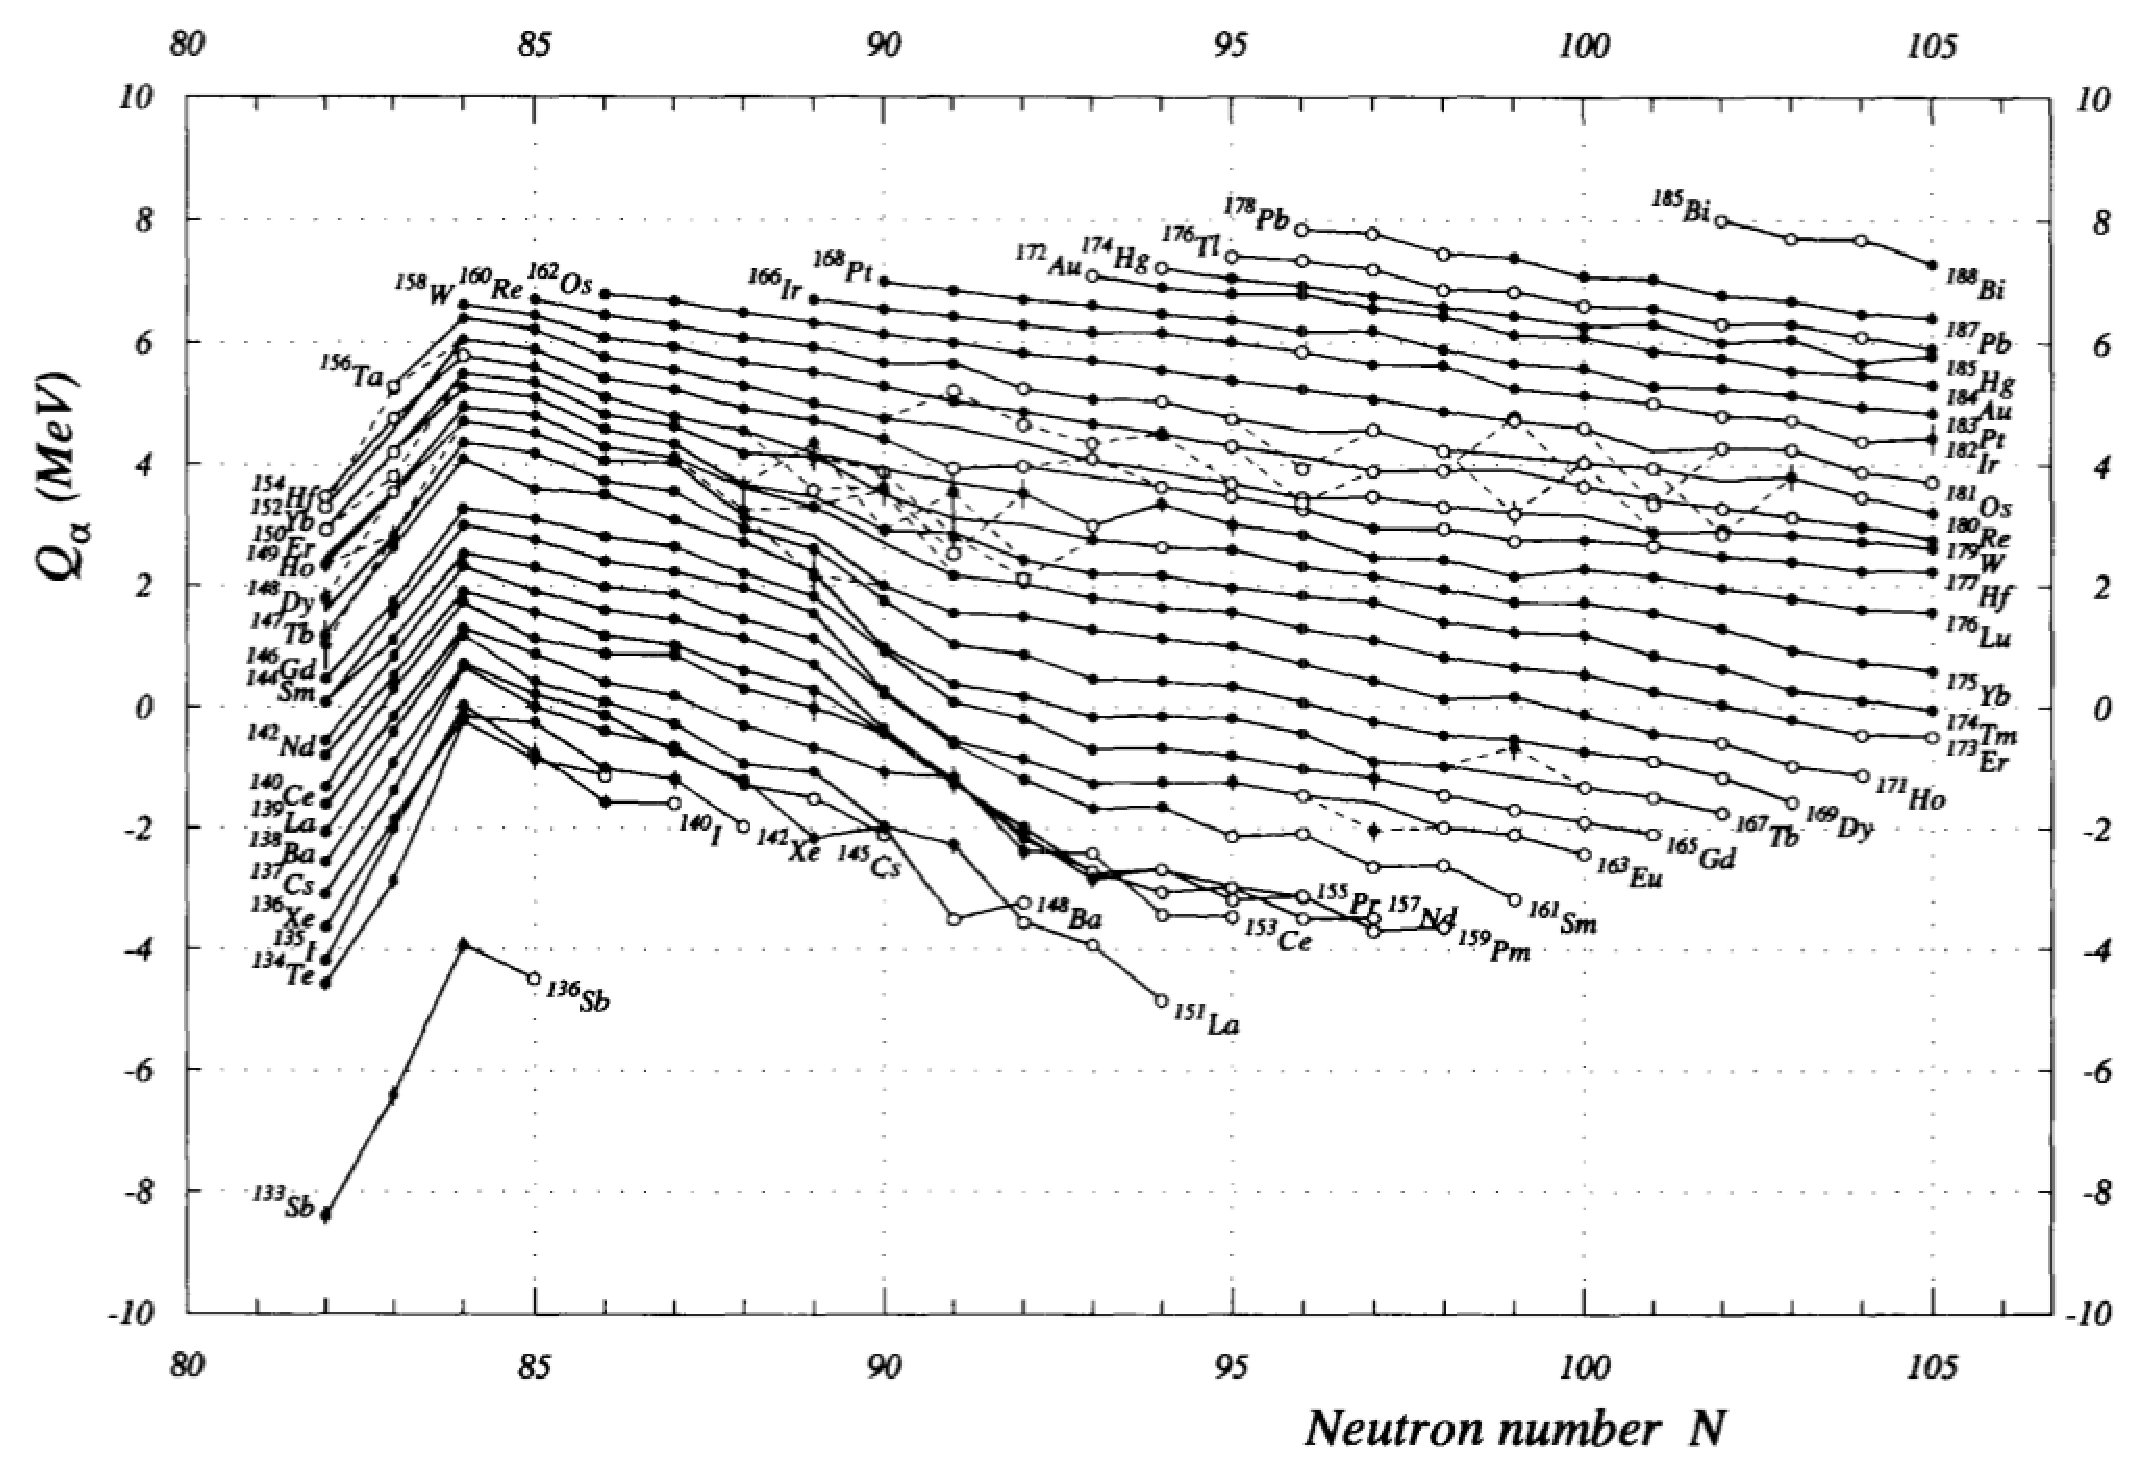
\includegraphics[width=0.8\textwidth]{figures/alphaSepEnergy.eps}
\caption[Alpha separation energy as an illustration of shell structure.]{Alpha separation energy as a function of neutron number.  The behavior around $N=84$ is indicative of shell structure.  From {\refref}~\cite{massEval_1993}.}
\label{fig:alphaSep}
\end{figure}
Such a structure is suggestive of that seen in atomic electrons, which experience a central potential primarily due to the Coulomb interaction.  Such a potential is not an appropriate model for nucleus, where the potential is known to be short range \citep{Casten}.  One model that has promising beginnings is the harmonic oscillator potential.  To determine the magic numbers predicted by this potential, consider the quantum numbers that describe an eigenstate of this potential.  The principal quantum number, $n$, indicates the number of nodes of the state.  In this work, the node at infinity is included rather than the node at zero, so that $n$ ranges from 1 to $\inf$.  The orbital angular momentum is denoted $l$, with $l = 0, 1, 2, 3, ...$ typically called the $s, p, d, f, ...$ orbitals as in atomic electron structure.  The eigenvalue associated with the projection of the orbital angular momentum operator along the $z$-axis is $m$, which varies between $-l$ and $l$ and is called the magnetic quantum number.  The eigenvalues of any eigenstate of a spherically symmetric potential cannot depend on the magnetic quantum number, so that for the harmonic oscillator potential, any state associated with $l$ has a multiplicity of $2(2l+1)$, where the additional factor of two is due to nucleons being spin-1/2 fermions.  The eigenvalues of the three-dimensional harmonic oscillator are $E_{nl} = (2n+l-\frac{1}{2})\hbar\omega$, so that the energies proceed in uniform steps as $2n+l$ increases by one unit.  {\fig}~\ref{fig:shellModelMagic} shows the level spacing for this potential; note that the energy levels are multiplets.  For example, the states $nl = 2s$ and $1d$ both have energy $\frac{3}{2}\hbar\omega$.  
\begin{figure}[htp]
\centering
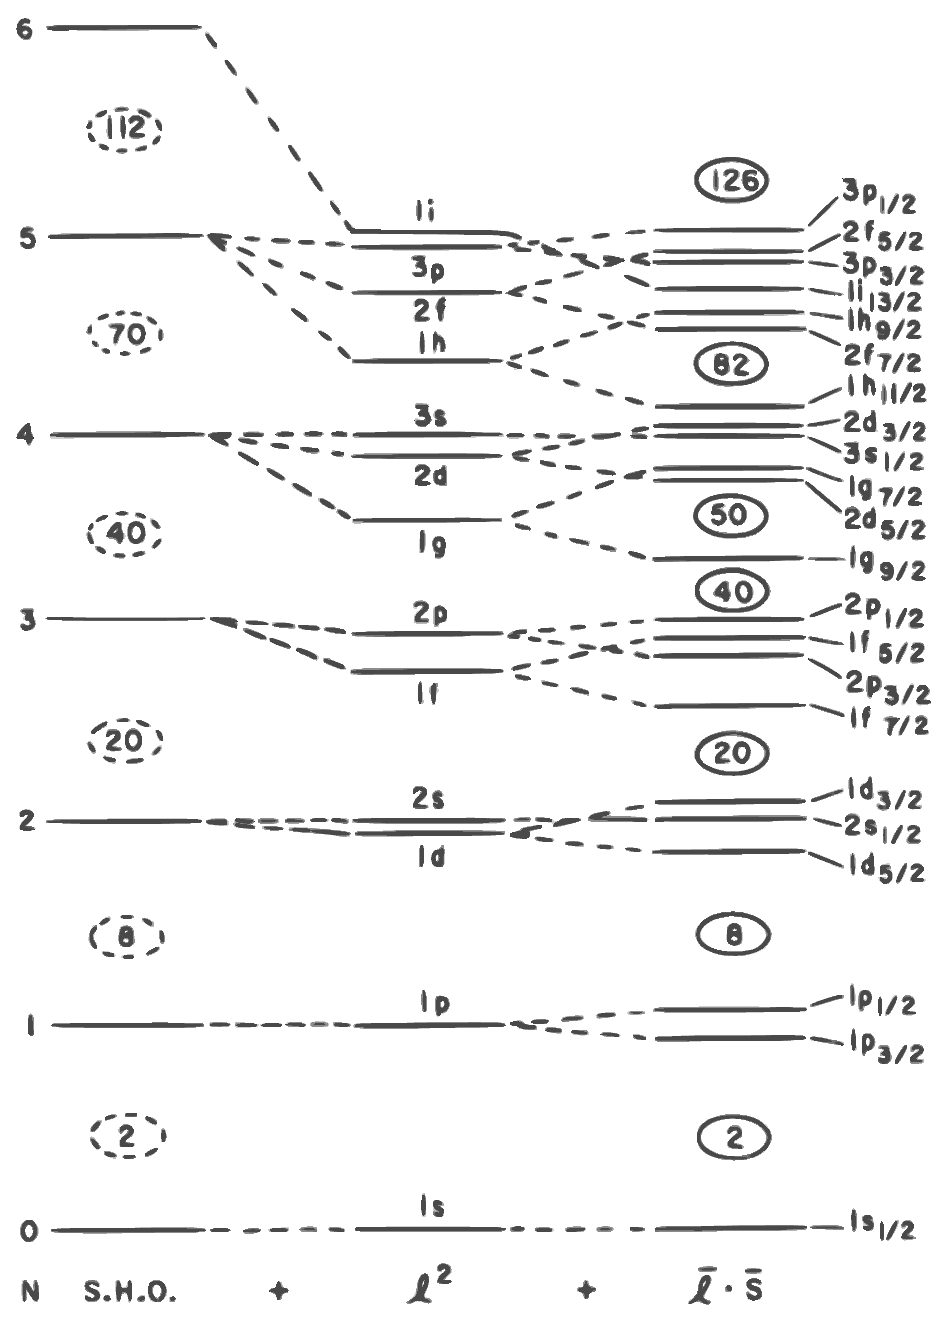
\includegraphics[width=0.8\textwidth]{figures/nuclearLevels.eps}
\caption[Level diagrams for different models of the nuclear Hamiltonian.]{Level diagrams for different models of the nuclear potential and their predicted magic numbers.  From left to right are the simple harmonic oscillator, a more flat-bottomed potential resulting from adding an $l^2$ term, and finally the addition of the spin-orbit coupling.  From {\refref}~\citep{Casten}.}
\label{fig:shellModelMagic}
\end{figure}
The harmonic oscillator potential predicts magic numbers at 2, 8, 20, 40, 70, and 112.  This matches the observed pattern for low numbers but begins to deviate for heavier nuclei.  A reasonable correction to make to the potential is to make it more uniform to more accurately reflect the fact that the density of nuclei is quite uniform \citep{Casten}.  Introducing a potential term proportional to $l^2$ does this by reducing the potential near the center of the well (where the orbital angular momentum is smaller) and increasing the potential further from the center, where the orbital angular momentum is larger.  Adjusting the potential in this way splits the $l$-degeneracy of the states but does not fundamentally change the predicted magic numbers.  It was not until Maria Goeppert-Mayer added a spin-orbit term to the potential \citep{MGM} that these magic numbers were correctly reproduced.  

Although the harmonic oscillator potential is useful in understanding many aspects of nuclear structure with the benefit of having well-understood quantum numbers, it has a number of shortcomings.  One has already been discussed - the bottom of the potential should be flatter to better describe the uniformity of nuclear matter.  This can be corrected by adding an $l^2$ term to the harmonic oscillator, but another approach is to define a new potential.  The Woods-Saxon potential \citep{WoodsSaxon} is a potential that reflects many of the known physical features of the nuclear potential and has the same quantum numbers as the modified harmonic oscillator potential described above.
\begin{figure}[htp]
\centering
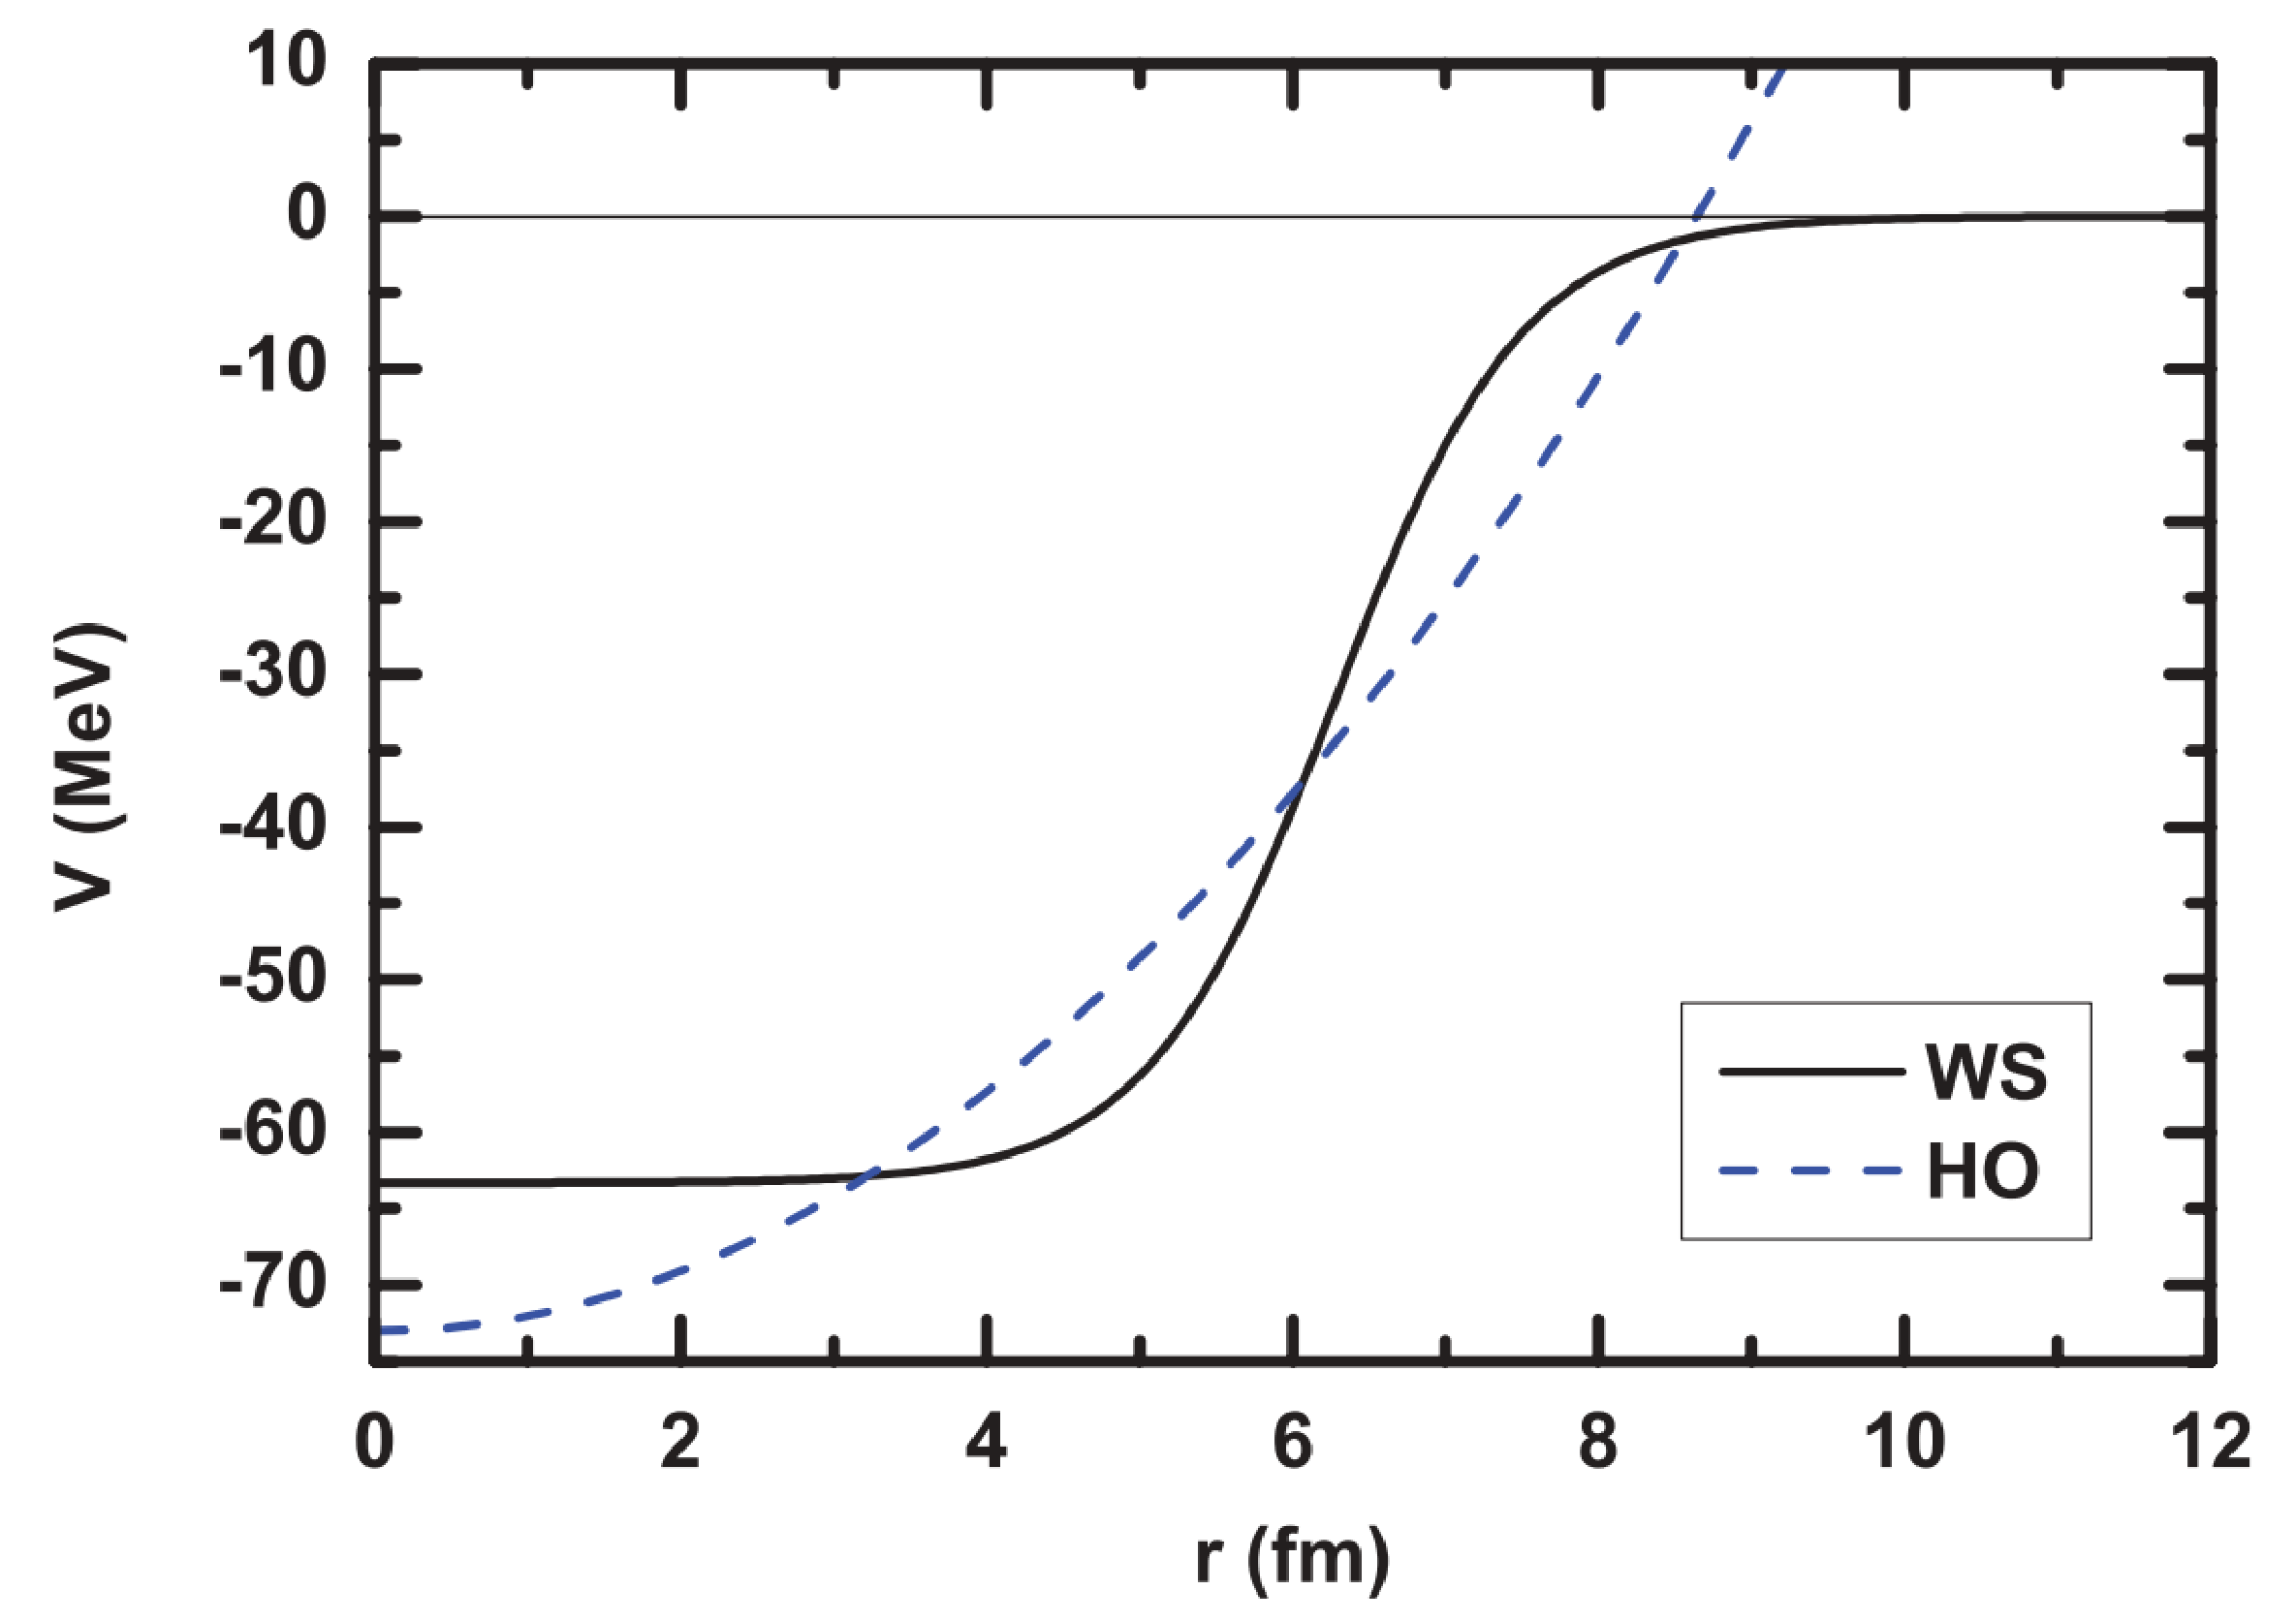
\includegraphics[width=0.8\textwidth]{figures/woodsSaxonVSharmonicOsc.eps}
\caption[The Woods-Saxon nuclear potential.]{A Woods-Saxon potential (solid line) compared to a pure harmonic-oscillator potential (dashed line).  Three parameters describe the Woods-Saxon potential: the well depth $V$, the radius $r_0$, and the surface diffusivity $a$.  Note that the Woods-Saxon potential drops to zero while the harmonic-oscillator potential increases without bound.  From {\refref}~\citep{pseudospinSymmetry}.}
\label{fig:woodsSaxon}
\end{figure}
The functional form of the Woods-Saxon potential is 
\begin{equation}
V(r) = \frac{V}{1+e^{(r-r_0)/a}},
\end{equation}
where $r$ is the distance from the center and the constants $V$, $r_0$, and $a$ represent the depth of the potential, the characteristic radius, and the surface diffusivity.  All further calculations discussed in this use this potential.

Understanding the nuclear potential is necessary but not sufficient to begin making predictions about nuclear behavior.  A nucleus consists of many nucleons, all moving within the nuclear potential and interacting with each other; one must describe this many-particle system.  A useful concept in nuclear structure is that of the valence shell of a nucleus.  Nucleons in a filled shell form a $J=0$ core that can be considered largely inert, while the remaining nucleons occupy the valence shell.  The picture is even further simplified due to the strong tendency for nucleons to couple into $J=0$ pairs, so that the ground state of a nucleus can be described simply by describing its unpaired nucleons.  The nucleus of primary interest in this work, \Se{76}, has 34 protons and 42 neutrons.  Like all even-even nuclei, its ground state is \zp, evidencing the strong coupling of nucleons into $J=0$ pairs.  The pairs studied by ($^3$He,n) transfer are proton-pair holes, whose valence shells are predicted to be $2f_{5/2}$.  While the phenomenological potentials discussed above reproduce trends in nuclear data with some accuracy, the exact wavefunctions of \SeProducts are not known and it can at best be said that the $f$, $p$, and $g$ orbitals are expected to be the primary components of the ground-state wavefunction.  Because the \NME depends on the overlap between the initial and final nuclei, it is desirable to understand these nuclei, and particularly the differences between their ground states, as accurately as possible.  A series of experiments were undertaken to understand these wavefunctions more accurately and will be discussed in {\sect}~\ref{sec:valence}.

\section{Calculation of \NME and Experimental Constraints}

One approach to calculating \NME = $\langle f||O||i \rangle$ is with the shell-model formalism described above.  The difficulty with this approach is that the \zvbb process is spatially confined to $\sim$2-3~fm, which means that intermediate states with excitation energies up to $\sim$100~MeV \citep{anatomy} are relevant to the calculation.  Even though expressing these states with a shell-model basis set can require a space as large as $O(10^{10})$,  several groups have still undertaken this method of calculating \NME \citep{CaurierShellModel}.  Regardless of the method of calculation, the wavefunctions of the initial and final nuclei must impact \NME.  Extensive single-nucleon transfer experiments have been performed to better understand the valence shells and are discussed further in {\sect}~\ref{sec:valence}.

A more common approach to the calculation of \NME is the Quasi-Particle Random-Phase Approximation (QRPA).  The QRPA is a density functional theory that provides a framework particularly suited for describing collective excitations \citep{Casten}.  QRPA assumes that the ground state of the nucleus is in a fully-paired state \citep{BenderSCMF} similar to that in descriptions of superconductivity described by Bardeen, Cooper, and Schreiffer (BCS) \citep{BCS}.  The BCS ground state for even-even nuclei was first suggested by Bohr and Mottelson \citep{nucleiBCS} and is still considered a good approximation for many nuclei \citep{validRegionsBCS_highMass}.  It is known, however, that BCS symmetry is not always a good approximation \citep{NambuBCS}.  In these cases, QRPA calculations can be inaccurate.  Two-nucleon transfer experiments can be helpful in determining the distribution of pairing strength in a nucleus \citep{Yoshida} and therefore support the QRPA assumption of a BCS-like ground state.  See {\sect}~\ref{sec:correlations} for more details on the effect of nuclear correlations on the calculation of \NME. 

\section{Valence Shells of the Initial and Final Nuclei}
\label{sec:valence}
\begin{comment}
\subsection{NME calculations and valence States}
\begin{itemize}
\item (assume that) NME calculations are sensitive to occupied valence states
\item can investigate valence state occupation with transfer reactions
\item \Ge{76} occupancies were experimentally determined and adjusting the energy levels to match changed the NME by a factor of 2 \citep{0vbbReview}
\end{itemize}
\end{comment}
As discussed in {\chap}~\ref{chap:0vbb}, the half-life of the \zvbb process depends on the participating nuclei as well as the neutrino mass scale.  While a direct measurement of \NME = $\langle f|O|i \rangle$ is difficult because it is only accessible by observation of \zvbb, it is possible to study the initial and final nuclear states separately in an attempt to improve the accuracy of the calculations.  

The initial and final nuclear states could inhibit \zvbb if there were significant rearrangement in the neutron or proton shell occupancies.  Single-nucleon transfer is sensitive to the occupancies and vacancies of valence nucleons and therefore an important tool in determining the extent to which the occupanices change between two nuclei.  Very generally, the cross section for transferring a nucleon to a specific shell in a target nucleus will be high if that nucleus has many holes available in that shell but low if that shell is filled.  The Macfarlane and French \citep{sumRules} sum rules state that the sum of occupancies and vacancies for an orbital with angular momentum $j$ must be $(2j+1)$.  This allows determination of valence shell occupancies and vacancies from experimental transfer data.  The validity of the sum rules was recently checked \cite{SumRulesTest} for Ni isotopes, whose valence orbitals are $f-p-g$ like \GeTargets.  

It should be noted that while there is extensive transfer-reaction data, it is not all suitable for determining valence shell occupancies because of uncorrelated systematic errors in the absolute cross-sections of complementary reactions.  Comprehensive single-nucleon transfer experiments that are specifically designed to limit these relative systematic errors have been performed on several of the candidate nuclei; see \citep{schiffer_review} for an overview of current progress.  In particular, the nuclei \GeTargets have been studied with the neutron-adding reactions (d,p) and ($\alpha$,\He{3}) as well as neutron-removing reactions (p,d) and (\He{3},$\alpha$) \citep{valenceNeutrons}.  The valence protons of these same nuclei have been studied with the (d,\He{3}) and (\He{3},d) reaction \citep{valenceProtons}.  These studies were done on the \Ge{74} and \Se{74} nuclei as a consistency check.  It was found that the Fermi surface of both the protons and neutrons in \GeTargets and \SeProducts are quite diffuse, with the relevant neutron and proton orbits being 2$p_{3/2}$, 1$f_{5/2}$, 2$p_{1/2}$, and 1$g_{9/2}$.  The quantities most important to the \NME calculations are the differences in occupancies between the mother and daughter nucleus; these differences are shown in {\fig}~\ref{fig:occupancyDiffs} along with the theoretical predictions.
\begin{figure}[!htbp]
\centering
\subfloat[][]{
   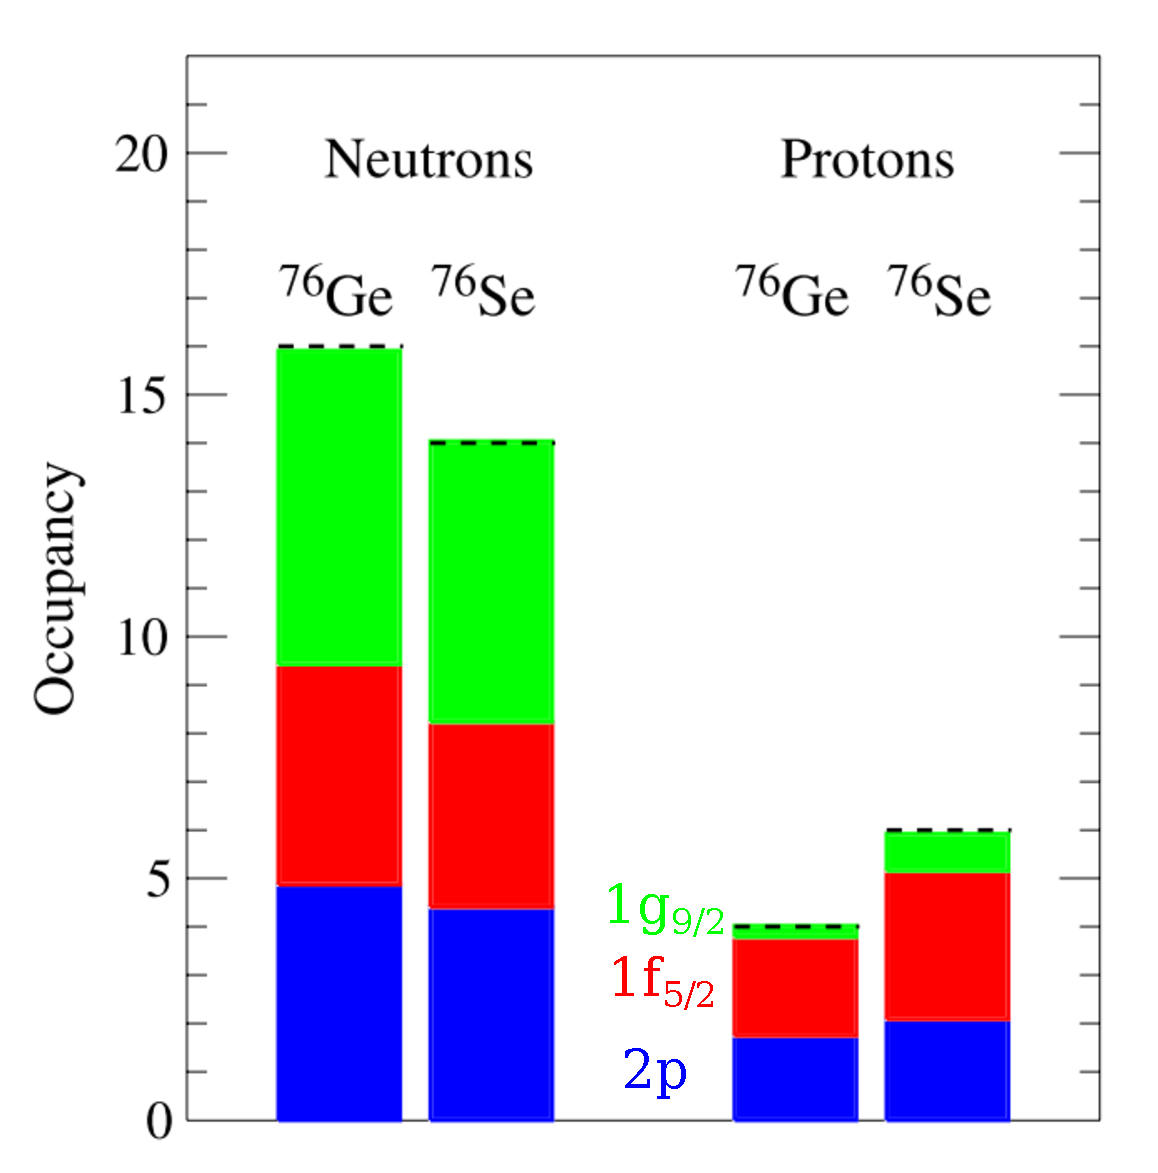
\includegraphics[width=0.4\textheight]{figures/occupancies.eps}
}
\\
\subfloat[][]{
   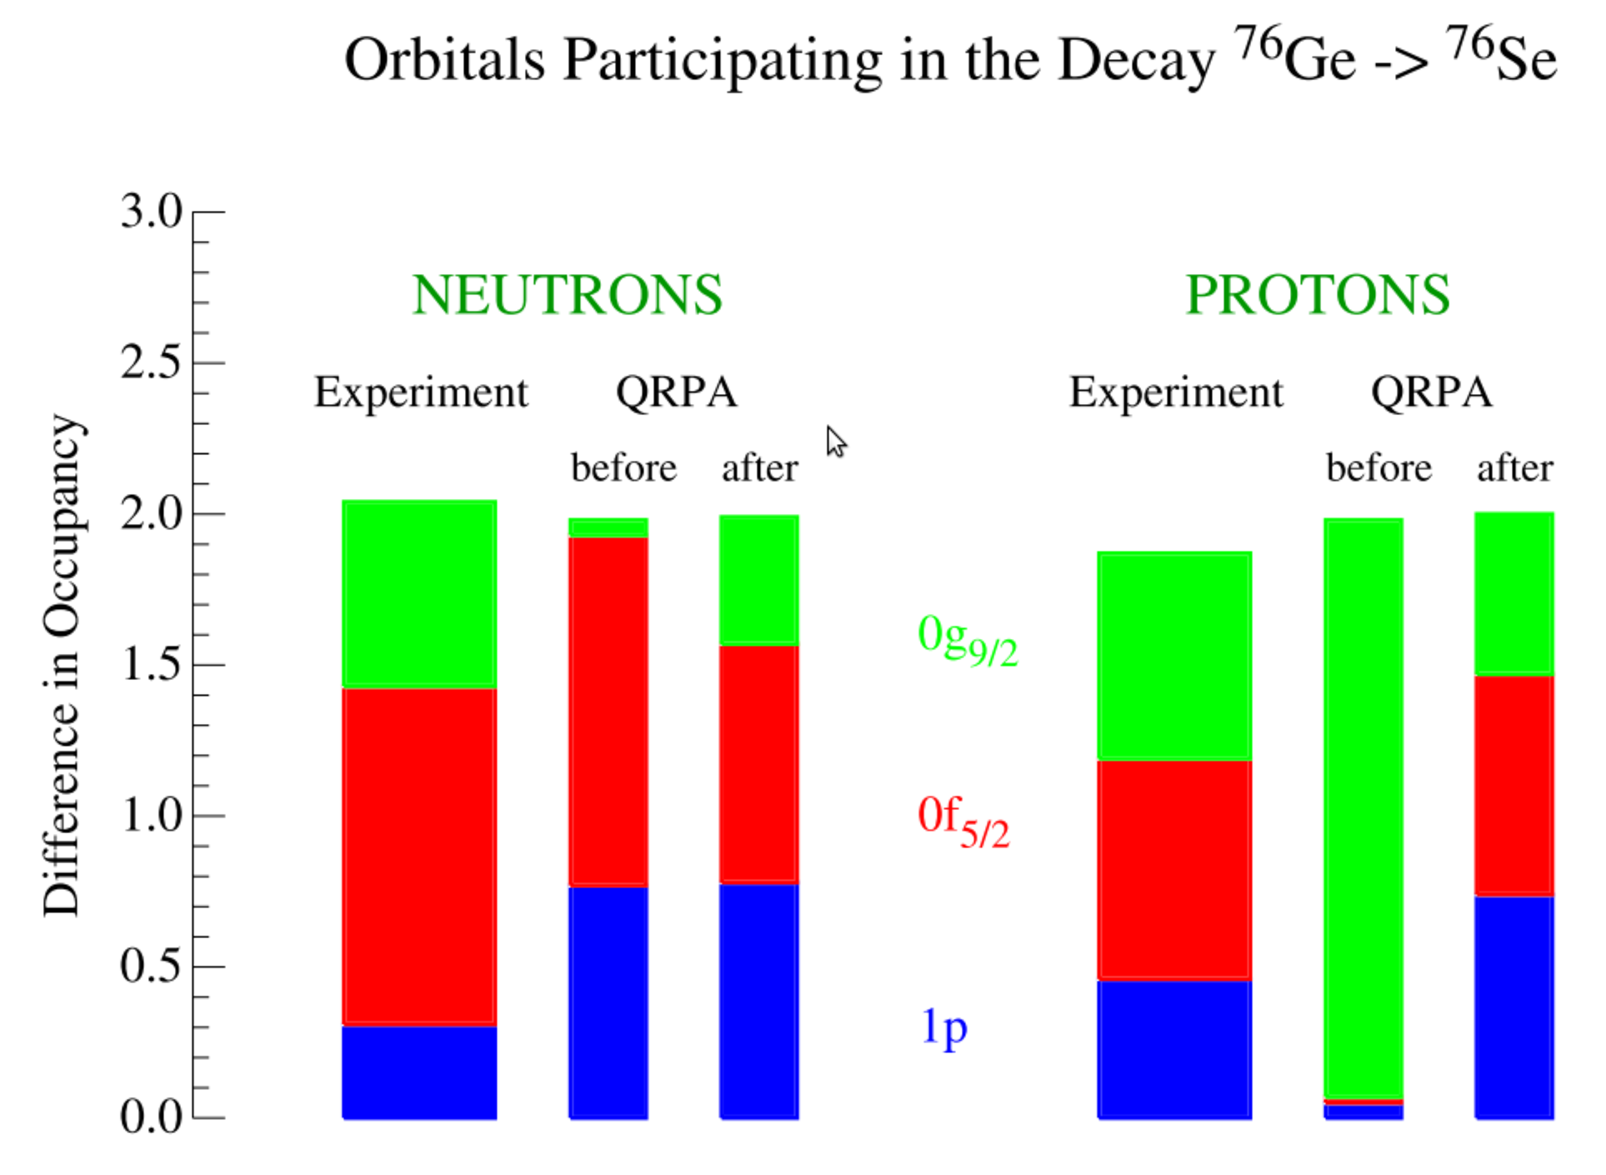
\includegraphics[width=0.5\textheight]{figures/occupancyDiffs.eps}
}
\caption[Occupancies of the neutron and proton valence shells of \Ge{76} and \Se{76}.]{(a) Occupancies of the neutron and proton valence shells of \Ge{76} and \Se{76} determined by single-nucleon transfer reactions.  From \citep{schiffer_review}.  (b)  The differences between occupancies in the final and initial states are determined from (a) and are more immediately relevant to \NME calculations.  The theoretical predictions, before and after adjusting level energies to better match the data, are shown next to the experimental values.  Modified from {\refref}~\citep{schiffer_review}.}
\label{fig:occupancyDiffs}
\end{figure}
The single-particle energy levels were adjusted in the QRPA calculation \citep{SuhonenEnergyAdjust} to provide better agreement with the data.  These changes reduced the QRPA calculation of \NME by approximately a factor of two, bringing it into agreement with the shell-model calculation of \NME.  This reduction in the spread of calculated \NME is particularly valuable to reducing the uncertainty of mass limits or estimates from \zvbb searches. 

\section{Nucleon-nucleon correlations and the impact they have on NME}
\label{sec:correlations}
\begin{comment}
\begin{itemize}
\item \zvbb occurs on correlated neutron pairs
\item certain pairing in the nucleus can inhibit \zvbb
\item investigate pair correlation with two-nucleon transfer reactions
\item some systems don't have all their \zp in the ground state - Xe
\item discuss neutron transfer experiments done on \GeTargets
\item wish to investigate proton transfer on \GeTargets
\end{itemize}
\end{comment}
In addition to studying the single-nucleon states in \GeTargets and \SeProducts, understanding correlated neutron pairs in \Ge{76} and correlated proton pair holes in \Se{76} is relevant to \NME.  Calculations suggest that significant contributions to \NME come from inter-nucleon distances of less than 3~fm \citep{anatomy}.  The distribution of highly-spatially-correlated \zp strength, therefore, may strongly influence \NME.  QRPA calculations can be particularly sensitive to \zp strength that is not exclusively in the ground state as these models assume a BCS approximation where the ground state contains all the \zp strength \citep{BenderSCMF}. 
transfered protons strongly populate pairing vibrationsticularly useful probes of pairing in nuclei as the transfered protons strongly populate pairing vibrations \citep{Yoshida}.  The cross section of a two-nucleon-transfer reaction on a nucleus that is well described by BCS should show strong population of the \zp ground-state with little, if any, population of \zp excited states.  A system that demonstrates the motivation for studying pairing in \Se{76} particularly well is $^{130}$Te, another candidate nucleus for \zvbb.  The neutron-pair (p,t) transfer reaction was used to show that the cross section for excited \zp states is less than 4\% of the ground-state yeild \citep{neutronPairsTellurium}, suggesting that BCS symmetry is a reasonable approximation for the neutrons in $^{128,130}$Te.  The same is not true for the proton states; the (\He{3},n) reaction populates an excited \zp state with a cross section that is $\sim$30\% of the ground-state cross section for both $^{128}$Te and $^{130}$Te \citep{protonPairsTellurium}.  Studies of \Ge{76}(p,t) and \Se{76}(p,t) show that the \zp strength is distributed overwhelmingly to the ground state, with excited-\zp states being populated at less than a few percent \citep{neutronPairsGermanium}.  As can be seen in $^{128,130}$Te, however, \zp strength distribution of the neutrons in a nucleus does not necessarily resemble that of the protons.  The aim of this work is to study the distribution of the proton-pair strength using the two-proton transfer reaction \reaction.  The \Ge{76} target servew as a check on the results obtained for \Ge{74}, which are the most relevant for \zvbb of \Ge{76}. 

\section{Modeling Two-Proton Transfers}
\begin{comment}
Discuss DWBA theory of two-proton transfer reactions
\begin{equation}
M\sim\langle\psi_n|V_T|\psi_{^3He}\rangle
\end{equation}
Where $V_T$ is the transfer operator and $\psi$ are elastic scattering wave functions.
Assume that nuclear elastic scattering is the largest contribution to the nuclear reaction and use 1st order perturbation theory to generate $V_T$ from the bound-state wave functions.
To get $\psi$ (?)
\begin{enumerate}
\item treat two particles individually
\item treat two protons as bound cluster
\end{enumerate}
treating particles individually is too complicated
when using cluster model, can adjust $V_0$ of well to match ?? binding energy and adjust $r_0$ to adjust range and $a_0$ to adjust ??.

cluster model's prediction of 0 degree cross section is sensitive to these parameters, but the relative cross sections of f-p-g shell nuclei do not depend strongly on the parameters.

Discuss experimental difficulties of two-proton transfer reactions and introduce NSL as a good place to do them
\end{comment}
Measuring differential cross sections can give information about underlying characteristics of nuclei.  For example, population of excited \zp states in two-nucleon transfer reactions gives information about pairing in a nucleus.  However, the calculated cross sections are also influenced by factors not related to nuclear pairing such as kinematics.  These contributions are not as relevent to the calculations of \NME as those that are sensitive to the pairing force.  The distorted-wave Born approximation (DWBA) is used to calculate cross sections of transfer reactions by assuming that nuclear elastic scattering is the largest contribution to the nuclear reaction and that the transfer operator can be constructed from the bound-state wavefunctions of the initial and final states using first-order perturbation theory.  This assumption is particularly accurate for the forward angles which are of interest in this experiment.

In general, four potentials are needed to perform a DWBA calculation in the case of a transfer reaction $(A = C+x)+B\rightarrow C+(D = B+x)$ where $x$ is transferred onto the nucleus $B$.  The potential felt by the incoming nucleus $A$ due to nucleus $B$ and the potential felt by the outgoing nucleus $C$ due to the product nucleus $D$ are both necessary.  The optical-model potentials are of the form
\begin{equation}
\begin{split}
U(r) = & V_C - Vf(x_0) + \left( \frac{h}{m_{\pi}c} \right) ^2 V_{SO}(\sigma\cdot l)\frac{1}{r}\frac{d}{dr}f(x_{SO}) \\
 & -i[Wf(x_W) - 4W_D\frac{d}{dx_D}f(x_D)],
\end{split}
\end{equation}
where $V_C$ is the coulomb potential and $f(x)=(1+e^x)^{-1}$ is the Woods-Saxon potential \citep{PereyPerey}.  The variable $x$ is defined as $(r-r_iA^{1/3})/a_i$, where $r$ is the distance from the center of the nucleus, $r_i$ is the reduced radius of a particular interaction, and $a_i$ describes the diffuseness.  The constants $h$, $m_{\pi}$, and $c$ are the Planck constant, the rest mass of the pion, and the speed of light, respectively.  Note that the functional form of the spin-orbit term $V_{SO}(\sigma\cdot l)$ is the derivative of the Woods-Saxon potential, making it predominantly a surface effect.  The imaginary component of the potential allows for absorbtion and, like the real part, has a volume term $W$ and, in addition, a surface term $W_D$.  The parameters of the optical-model potentials are determined by fits to elastic scattering data.  Parameter sets that are in common use, such as the Becchetti-Greenlees neutron potential \citep{Becchetti_neutronPotential}, are global fits to large sets of data \citep{PereyPerey}.  Potentials to bind the transfer nucleons to its original nucleus $C$ and final nucleus $B$ are also needed. 
When calculating proton-pair transfer cross sections, this method can be complicated considerably when treating each proton in the pair separately.  This approach is that of Bayman and Kallio \citep{BaymanKallio}, which can accurately predict the absolute differential cross section but also introduces additional parameters such as phases between multi-step transitions.  The many parameters needed to make this calculation are poorly constrained unless the wavefunction is well-understood beforehand.  A simpler method, the cluster model, treats the protons as a single, bound cluster.  While this method does not typically reproduce absolute cross sections well, it reproduces the angular distribution of the more-complicated Bayman-Kallio approach, as well as the experimental data.  It should be noted that, when using the either model to predict cross sections, their magnitudes are quite sensitive to the parameters in the Woods-Saxon potential, $r$ and $a$, which describe the radius of the well and the diffuseness of the surface, respectively.  However, the trend of the cross section relative to the energy of the incoming \He{3} or changing neutron number of the target is well-reproduced.

One can use DWBA calculations to understand the kinematic dependence of the expected cross section, as shown in {\fig}~\ref{fig:optimizeCrossSection}; this helps determine an appropriate beam energy.  
\begin{figure}[htp]
\centering
\includegraphics[width=1.0\textwidth]{figures/74Ge_0plus_xsection.eps}
\caption[The $^{74}$Ge($^3$He,n) \zp cross section at zero degrees as a function of beam energy.]{A plot showing the $^{74}$Ge($^3$He,n) \zp cross section at zero degrees as a function of beam energy.  From \citep{schiffer_privateCommunication}.}
\label{fig:optimizeCrossSection}
\end{figure}
It can be seen from this plot that the ideal beam energy for maximizing the \reaction cross section is slightly more than 18~MeV.  However, detector resolution decreases with increasing beam energy as discussed in {\sect}~\ref{sec:detector}.  Because the product nuclei \SeProducts have low-lying excited \tp states that could be populated with similar cross section to the ground state, the lower beam energy of 16~MeV was chosen to provide sufficient resolution for resolving these states.  See {\fig}~\ref{fig:levelDiagrams} for level diagrams of the product nuclei.
\begin{figure}[!htbp]
\captionsetup[subfloat]{labelformat=empty}
\centering
\subfloat[][]{
   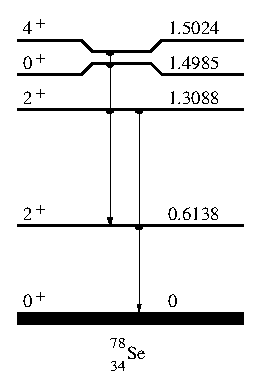
\includegraphics[width=0.3\textwidth]{figures/78Ge_levels.eps}
}
\hspace{2cm}
\subfloat[][]{
   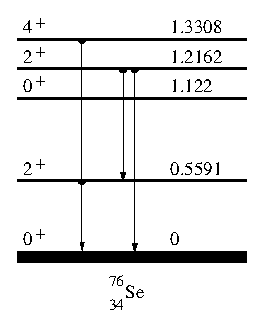
\includegraphics[width=0.3\textwidth]{figures/76Ge_levels.eps}
}
\caption[Level diagram of \Se{78} and \Se{76}.]{The level diagrams of the product nuclei, \Se{78} and \Se{76}.  Note the low-lying 2$^+$ state.  Notice also that both nuclei have known \zp levels.  These levels have been measured through $\gamma$-ray experiments.  Such experiments are not sensitive to the pairing in ground-state nuclei, which is why two-nucleon transfer reactions on \zvbb candidate nuclei are of such interest.}
\label{fig:levelDiagrams}
\end{figure}
As can be seen in {\fig}~\ref{fig:levelDiagrams}, there are known \zp states in \SeProducts.  However, these states were discovered through beta decay and excitation due to single-nucleon scattering \citep{NNDC}, neither of which gives information on the distribution of the paired \zp strength between these excited states and the ground state of \GeTargets.  That the leading method of calculating \NME relies on the assumption that the \zp strength is concentrated entirely in the ground state provides strong motivation to experimentally determine this distribution using two-proton transfer.  Particulars of the beam and neutron detector are discussed in {\chap}~\ref{chap:2pExpt} and an analysis of the results in {\chap}~\ref{chap:dataAnalysis}.
% % uncomment the following lines,
% if using chapter-wise bibliography
%
% \bibliographystyle{ndnatbib}
% \bibliography{example}
